\documentclass[tikz,border=3pt]{standalone}
% \usetikzlibrary{arrows.meta}
\usetikzlibrary{decorations.text}
\definecolor{mygray}{RGB}{143,188,143}
\definecolor{boxgray}{RGB}{200,200,200}

\definecolor{testblue}{RGB}{200,200,200}
\definecolor{designyellow}{RGB}{200,200,200}

\definecolor{darkgreen}{RGB}{0,100,0}
\newcommand*{\mytextstyle}{\sffamily\Large\bfseries\color{black!85}}

\newcommand*{\boxtextstyle}{\sffamily\small\bfseries\color{black!85}}
\newcommand{\arcarrow}[3]{%
   % inner radius, middle radius, outer radius, start angle,
   % end angle, tip protusion angle, options, text
   \pgfmathsetmacro{\rin}{1.7}
   \pgfmathsetmacro{\rmid}{2.2}
   \pgfmathsetmacro{\rout}{2.7}
   \pgfmathsetmacro{\astart}{#1}
   \pgfmathsetmacro{\aend}{#2}
   \pgfmathsetmacro{\atip}{5}
   \fill[mygray, very thick] (\astart+\atip:\rin)
                         arc (\astart+\atip:\aend:\rin)
      -- (\aend-\atip:\rmid)
      -- (\aend:\rout)   arc (\aend:\astart+\atip:\rout)
      -- (\astart:\rmid) -- cycle;
   \path[
      decoration = {
         text along path,
         text = {|\mytextstyle|#3},
         text align = {align = center},
         raise = -1.0ex
      },
      decorate
   ](\astart+\atip:\rmid) arc (\astart+\atip:\aend+\atip:\rmid);
}
\begin{document}
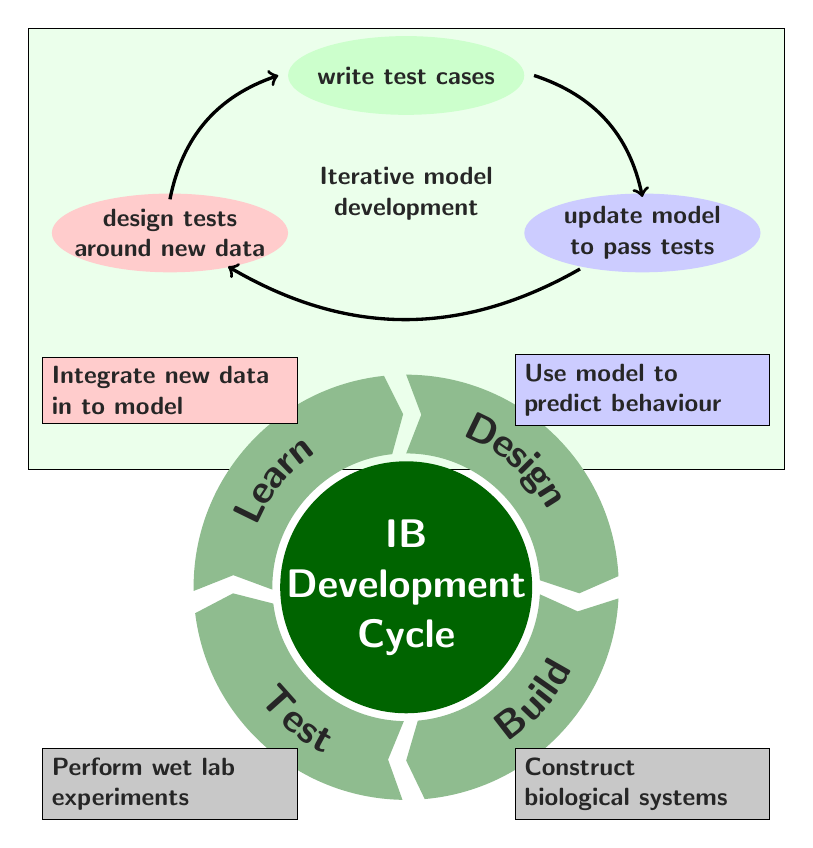
\begin{tikzpicture} %[>={Triangle[width=5mm,length=5mm]},->]
    
     \fill[even odd rule,green!8, draw=black] (-4.8, 7.1) rectangle (4.8,1.5);
    
    \node[
        text width = 5cm,
        font=\boxtextstyle,
        align=center] at (0, 5) {Iterative model \\ development};
    
    \fill[even odd rule,green!20] (0, 6.5) ellipse (1.5cm  and 0.5cm);
    \node[
        text width = 3cm,
        font=\boxtextstyle,
        align=center] (test) at (0, 6.5) {write test cases};
    
    \fill[even odd rule,blue!20] (3, 4.5) ellipse (1.5cm and 0.5cm);
    \node[
        text width = 3cm,
        font=\boxtextstyle,
        align=center
        ] (model) at (3, 4.5){update model to pass tests};
    
    \fill[even odd rule,red!20] (-3, 4.5) ellipse (1.5cm  and 0.5cm);
     \node[text width = 3cm, font=\boxtextstyle, align=center] (data) at (-3, 4.5)
     {design tests around new data};
    

    \path [->,very thick]  (model) edge[bend left] (data);
    \path [->,very thick] (data.north) edge[bend left] (test.west);
    \path [->,very thick] (test.east) edge[bend left] (model.north);
    
    
   \fill[even odd rule,darkgreen] circle (1.6);
   \node at (0,0) [
      font  = \mytextstyle,
      color = white,
      align = center
   ]{
        IB \\
      Development \\
      Cycle
   };
   \arcarrow{ 85}{  3}{Design}
   \arcarrow{270}{357}{Build}
   \arcarrow{182}{269}{Test}
   \arcarrow{176}{ 96}{Learn}
    
    %design
    \node[fill=blue!20, text width = 3cm,draw=black]  at (3,2.5)[
      font  = \boxtextstyle,
      align = left](design)
      {Use model to \\ predict behaviour};
      
%     \path [dashed] (design.north) edge (model.south);
    
    \node[fill=boxgray, text width = 3cm, draw=black] at (3,-2.5)[
      font  = \boxtextstyle,
      align = left]{Construct \\ 
        biological systems};

    \node[fill=boxgray, text width = 3cm, draw=black] at (-3,-2.5)[
      font  = \boxtextstyle,
      align = left]{Perform wet lab \\ 
      experiments};
    
    % learn
    
    \node[fill=red!20, text width = 3cm, draw=black]  at (-3, 2.5) [
      font  = \boxtextstyle,
      align = left] (learn) {Integrate new data\\ in to model};
    
%     \path [dashed] (learn.north) edge (data.south);


\end{tikzpicture}
\end{document}
